\documentclass[../main.tex]{subfiles}
% DOCUMENT

\begin{document}
\frontmatter
\pagestyle{empty}
\mainmatter
\pagestyle{fancy}
\chapter{Mô tả bài toán}\label{problem-description}

Cho một đồ thị có hướng \(D = (N, A)\), trong đó: \(N = {1, 2, ..., n}\)
là tập đỉnh và \(A \subseteq N \times N\) là tập cạnh; khung thời gian
\([0, T]\) và các hàm thời gian di chuyển tuyến tính từng khúc
\(c_{i,j}(t) > 0\) với \(t \in [0, T]\) thỏa mãn tính chất FIFO cho mọi
cạnh \((i, j) \in A\).\\
Tính chất FIFO, trong hàm tuyến tính, có nghĩa là
\textbf{độ dốc của các khúc ít nhất phải là \(-1\).} Không mất tính tổng
quát, ta luôn đi từ đỉnh nguồn \(1\) và kết thúc ở đỉnh đích
\(n\).

Đường đi
\(P=((i_1^P, t_1^P), (i_2^P, t_2^P), \dots, (i_{m(P)}^P, t_{m(P)}^P))\)
là một dãy gồm \(m(P)\) cặp đỉnh - thời gian, trong đó dãy các đỉnh
\((i_1^P, i_2^P, \dots, i_{m(P)}^P)\) tạo thành đường đi trong đồ thị
\(D\) từ \(i_1^P\) đến \(i_{m(P)}^P\), và mỗi nút trong dãy \(i_k^P\)
tương ứng với thời gian \(t_k^P\), đại diện cho thời gian bắt đầu di
chuyển trên cạnh \((i_k^P, i_{k+1}^P)\) với \(k=1, \dots m(P)-1\). Riêng
đỉnh \(i_k^P\) với \(k=m(P)\) biểu diễn thời gian đến đích. Do đó dãy
các cặp cần thoả mãn tính chất:
\[t_{k+1}^P \ge t_k^P + c_{i_k^P, i_{k+1}^P}(t_k^P)\] với
\(k=1, \dots m(P)-1\). Nếu
\(t_{k}^P \ge t_{k-1}^P + c_{i_{k-1}^P, i_{k}^P}(t_{k-1}^P)\) với bất kì
\(k \ge 2\), (hoặc nếu \(t_1^P > 0\)), thì ta nói rằng đỉnh \(i_k^P\)
cần phải đợi.\\ 
Nếu \(t_{k}^P = t_{k-1}^P + c_{i_{k-1}^P, i_{k}^P}(t_{k-1}^P)\) với mọi
\(k \ge 2\) thì ta nói rằng \(P\) không có chờ đợi (waiting-free). \\
Nếu \(P\) bắt đầu tại đỉnh \(i_1^P = 1\) với \(t_1^P\ge0\) và kết thúc tại
đỉnh \(i_{m(P)}^P=n\) với \(t_{m(P)}^P \le T\) thì ta nói \(P\) là một
đường đi khả thi. Ta kí hiệu \(\mathcal{P}\) biểu diễn tập hợp tất cả các
đường đi khả thi như vậy.

Ba hàm mục tiêu chính được quan tâm ở đây là:

\begin{enumerate}
\def\labelenumi{\arabic{enumi}.}
\tightlist
\item
  \textbf{Tối thiểu thời gian đến đích:}
  \[\min_{P\in \mathcal P}t_{m(P)}^P\]
\item
  \textbf{Tối thiểu thời gian thực hiện (đi từ nguồn đến đích):}
  \[\min_{P\in \mathcal P}(t_{m(P)}^P-t_1^P)\]
\item
  \textbf{Tối thiểu tổng thời gian di chuyển trên các cạnh của đường đi
  từ nguồn đến đích:}
  \[\min_{P\in \mathcal P}\sum_{k=1}^{m(P)-1}c_{i_k^P, i_{k+1}^P}(t_k^P)\]
\end{enumerate}

Trong phần còn lại của bài luận, tôi sẽ bỏ đi chữ \(P\) ở trên các đỉnh cùng một đường đi để thuận tiện cho ký hiệu và dễ nhìn
hơn.

Để minh họa ba hàm mục tiêu này, hãy xem xét đồ thị (a) và các hàm thời
gian di chuyển (b,c,d) trong \autoref{fig:1}, với \(n = 3\) và khung thời gian
cho trước là \([0, 4]\).

\begin{itemize}
\tightlist
\item
  \textbf{Đường đi tối thiểu thời gian đến đích} là
  \(((1, 0), (3, 3.5))\): Xuất phát tại thời điểm \(t = 0\), đi qua cạnh
  \((1, 3)\) và đến đích tại \(t = 3.5\), giá trị hàm mục tiêu là
  \(3.5\).
\item
  \textbf{Đường đi tối thiểu thời gian thực hiện} là
  \(((1, 1.5), (2, 3), (3, 4))\): đường đi bắt đầu từ \(t = 1.5\), đi
  qua cạnh \((1, 2)\) và đến đỉnh \(2\) tại \(t = 3\). Sau đó bắt đầu từ
  \(t = 3\), đi qua cạnh \((2, 3)\) và đến đỉnh đích tại \(t = 4\), giá
  trị mục tiêu là \(2.5\). Vì không phải chờ đợi trên đường đi này nên
  tổng thời gian di chuyển cũng là \(2.5\).
\item
  Tuy nhiên, đường đi trên không cho ra tổng thời gian di chuyển trên
  các cạnh là tối thiểu. Có nhiều nghiệm tối ưu cho bài toán này. Đối
  với \(t_1 \in [0, 1]\) bất kỳ, đường đi \(((1, t_1), (2, 3), (3, 4))\)
  có thời gian di chuyển tối thiểu: nó sẽ đi qua cạnh \((1, 2)\), bắt
  đầu từ thời gian \(t_1\) và đến hết cạnh tại \(t_1 + 1 \in [1, 2]\),
  sau đó chờ tại đỉnh \(2\) cho đến \(t = 3\) và đi qua cạnh \((2, 3)\)
  tại \(t = 4\), mang lại giá trị mục tiêu là \(2\).
\end{itemize}

\begin{figure}[H]
\centering
% 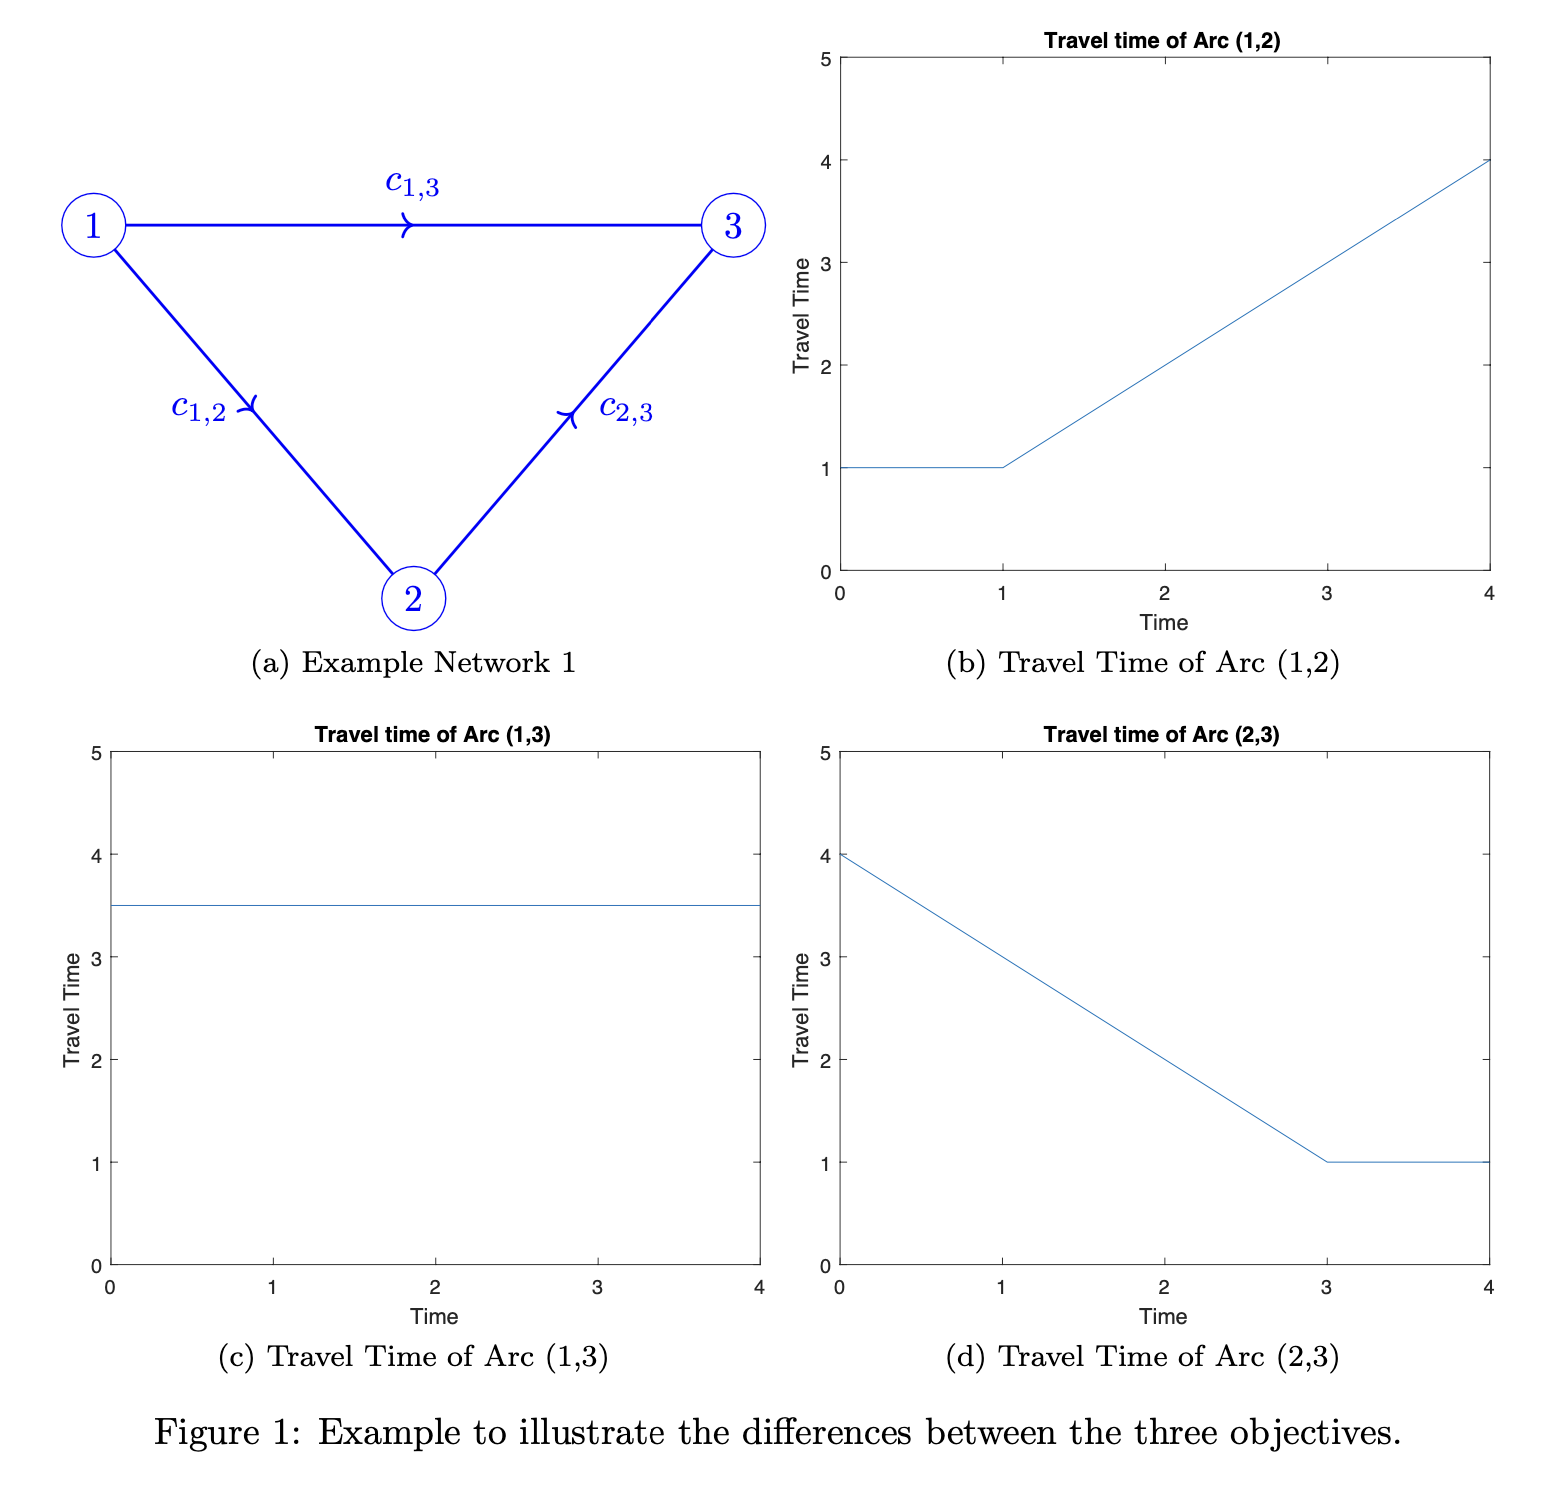
\includegraphics{images/Figure1.png}
\subcaptionbox{Mạng lưới \(1\)\label{fig:1a}}{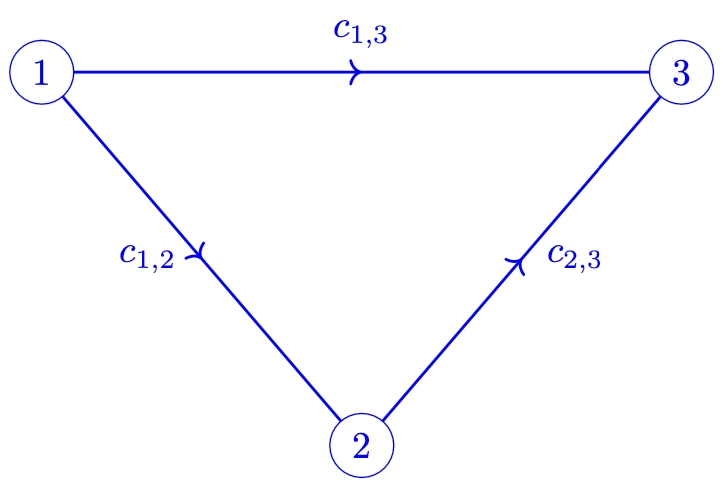
\includegraphics[width=.45\textwidth]{edited-images/Figure1a.jpg}}
\subcaptionbox{Cung \((1, 2)\)\label{fig:1b}}{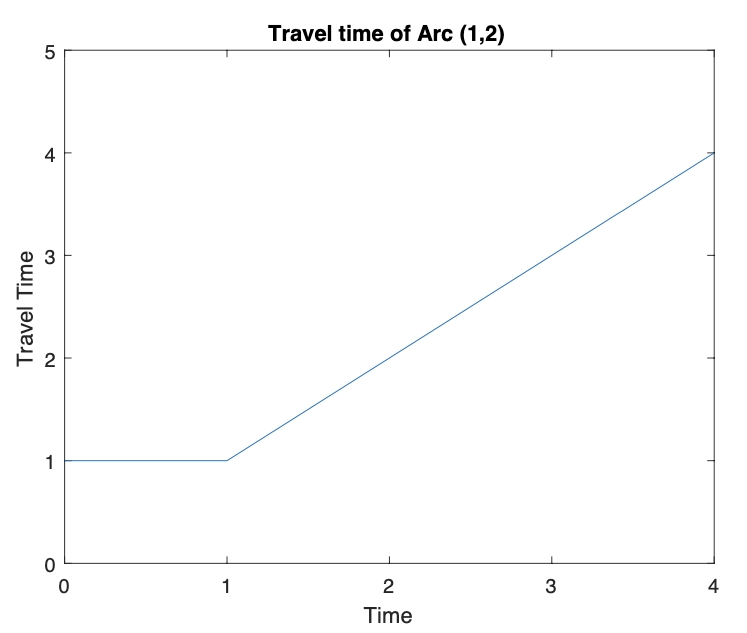
\includegraphics[width=.45\textwidth]{edited-images/Figure1b.jpg}}
\subcaptionbox{Cung \((1, 3)\)\label{fig:1c}}{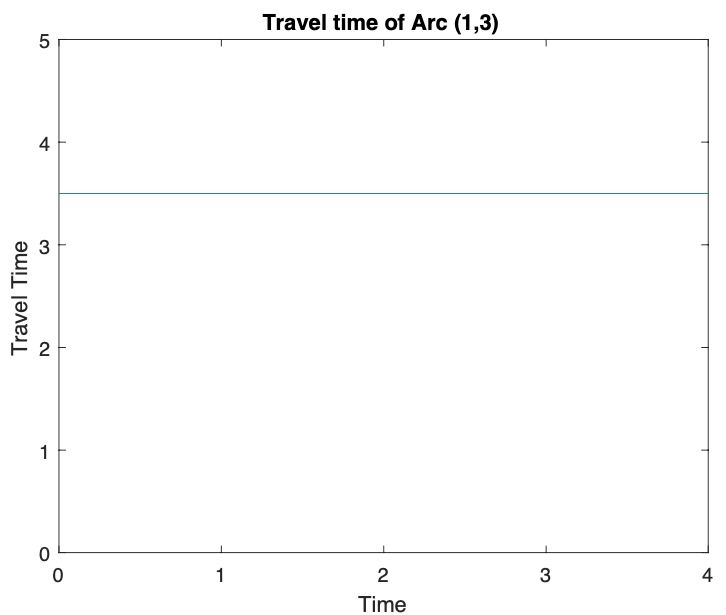
\includegraphics[width=.45\textwidth]{edited-images/Figure1c.jpg}}
\subcaptionbox{Cung \((2, 3)\)\label{fig:1d}}{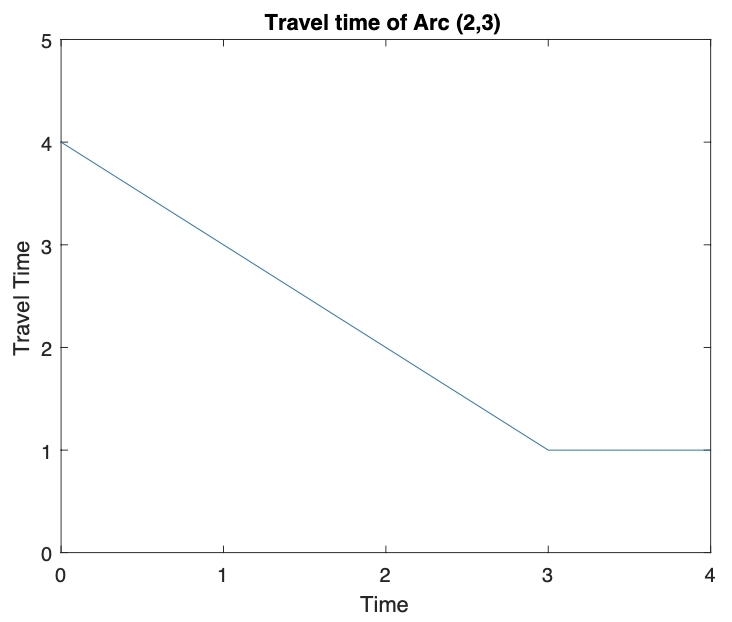
\includegraphics[width=.45\textwidth]{edited-images/Figure1d.jpg}}

\caption{Minh họa các hàm thời gian di chuyển}
\label{fig:1}
\end{figure}

Vì các hàm thời gian di chuyển có tính chất FIFO, khi giảm thời gian di
chuyển đến đích hoặc thời gian thực hiện, đường đi tối ưu luôn thỏa mãn
tính chất \(t_k + c_{i_k, i_{k+1}}(t_k) = t_{k+1}\) với
\(k = 1, \dots, m(P)-1\). Như đã đề cập ở trên, nghiệm tối ưu sẽ không
xuất hiện chờ đợi. Ngoài ra, khi giảm thời gian đến đích, đường đi tối
ưu sẽ có \(t_1^P = 0\).

Ba bài báo \cite{cooke1966shortest}, \cite{orda1990shortest}, \cite{dean2004shortest} đã đưa ra phương pháp
cho bài toán tìm đường đi đến đích sớm nhất có thể,  xuất phát tại đỉnh nguồn với thời gian cố định. 
Phương pháp này có độ phức tạp đa thức bằng cách mở rộng thuật toán tìm đường đi ngắn nhất
tiêu chuẩn. Tương tự áp dụng với bài toán tìm đường đi 
xuất phát từ nguồn muộn nhất có thể, đến đích với thời gian cố định.
Bằng cách tính trước các hàm thời gian di chuyển \emph{đảo chiều}: Với
cạnh \((i, j)\) và thời gian \(t\), hàm \emph{đảo chiều} được tính toán
tại \(t\) sẽ cho ra thời gian di chuyển \(\tau\) để kết quả thời gian
đến đỉnh \(j\) là \(t-\tau\). Ý tưởng này dẫn đến việc giải bài toán
TDSPP với nghiệm là đường đi ngắn nhất TDSP ở các phần sau.
\backmatter
\end{document}
% END DOCUMENT